\section{EXPERIMENTAL SETUP}
Data acquisition was conducted at Pouliot Pavilion of Laval University beginning February 11 and ending March 21. The sensors were placed close to the inner wall of a window facing N\SI{50}{\degree}E. A wooden structure held the LiDARs side by side at approximately \SI{13.9}{\meter} above the ground and the main scanning plane (i.e. \SI{0}{\degree} in the sensor reference frame) forming a \SI{30}{\degree} angle with respect to the building wall. In this configuration, a slight opening of the window allowed to keep the LiDARs inside while scanning outside. To avoid direct light exposure between sensors, corrugated plastic layers were placed between them. Note that we observed no interference between the sensor readings. Figure~\ref{fig:setup} present an overview of the setup.

\begin{figure}[h]
    \centering
    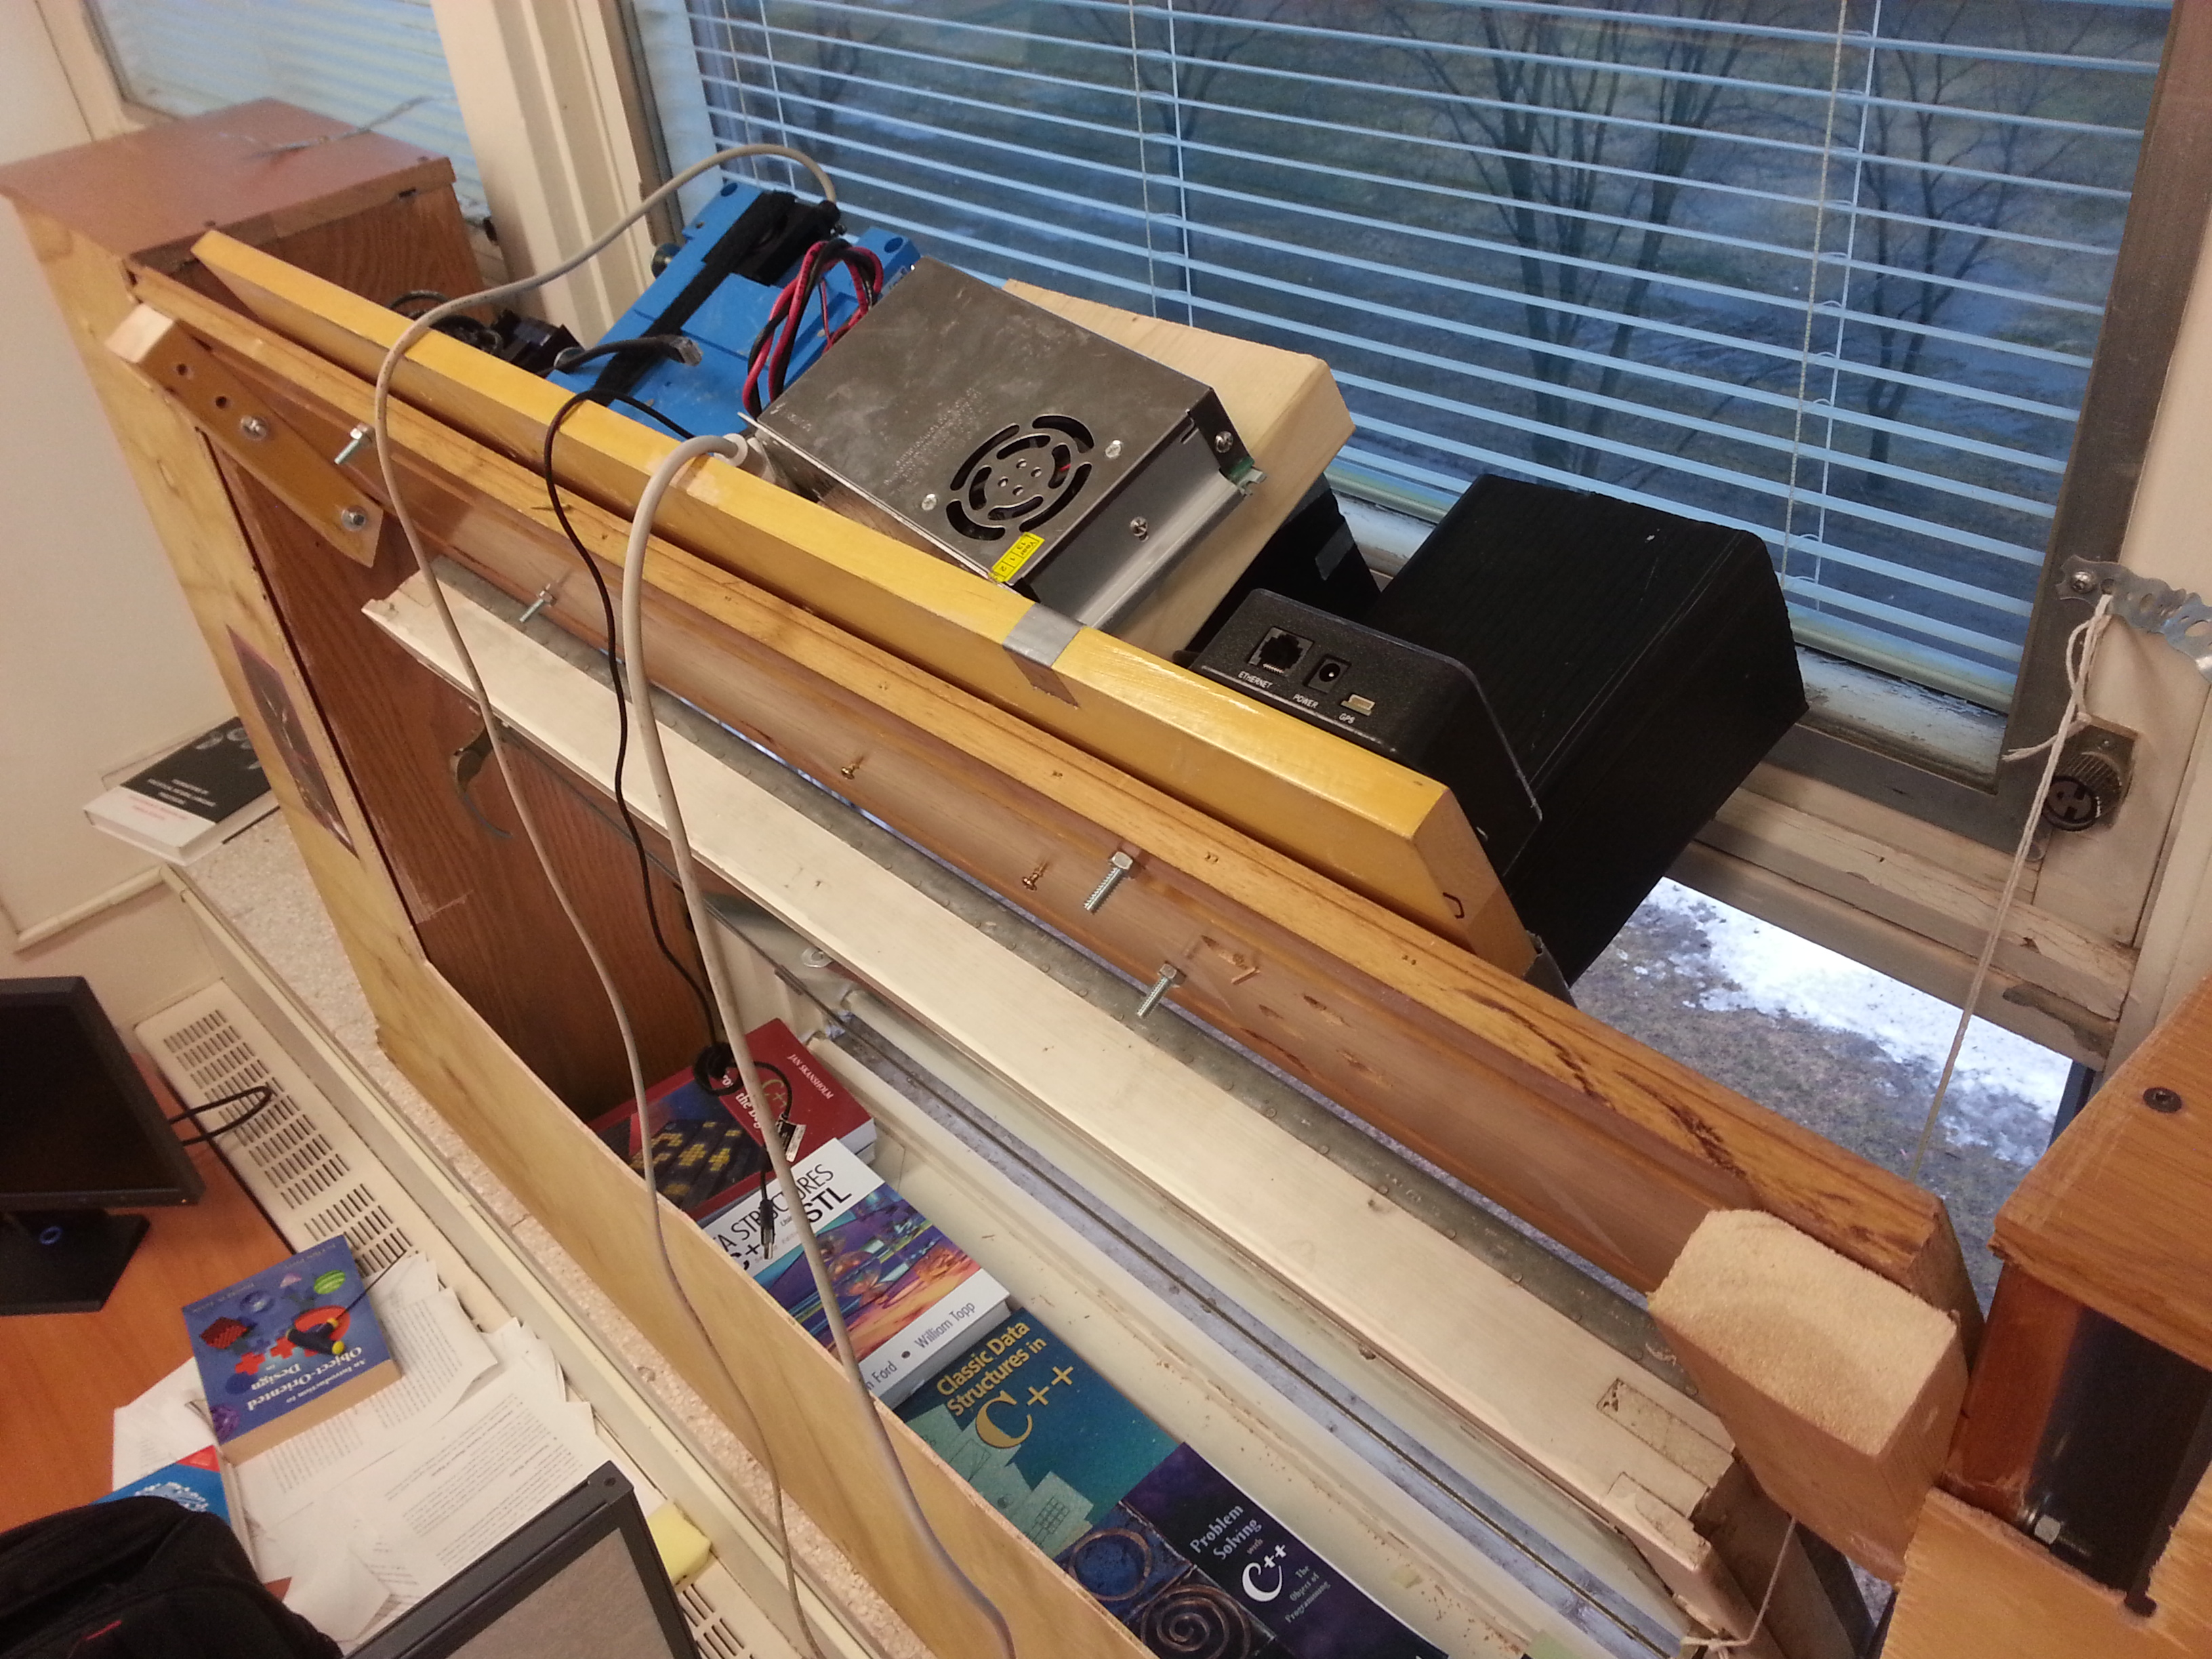
\includegraphics[width=0.95\linewidth]{./img/setup_diag.png}
    \caption{The experimental setup}
    \label{fig:setup}
\end{figure}

Means that in the building shadow from time to time.

%Some notes to fill up the table:
%\begin{itemize}
    %\item LMS200
        %\begin{itemize}
            %\item See page 8. Range vs reflectivity
            %\item See page 7. It is around 20cm at 20m
        %\end{itemize}
    %\item LMS151
        %\begin{itemize}
            %\item See page 25. Scanning range up to 50 m (164.04 ft) with $>$ 75\% object remission (18 m (59.06 ft) with 10\% object remission)
            %\item See page 26. $distance(mm (in)) * 0.015 rad + 8 mm (0.31 in)$
        %\end{itemize}
    %\item Hokuyo
        %\begin{itemize}
            %\item 0.1 to 10m : $\pm$30mm,10 to 30m : $\pm$50mm(White Kent Sheet)
            %\item See article : Spot size is 50 mm × 500 mm at sensor’s maximum distance of 30 m
            %\item See page 6. Up to 3 echoes.
        %\end{itemize}
    %\item Velodyne
        %\begin{itemize}
            %\item See manual page 12. 1 to 70 meters... Datasheet says 80-100m...
            %\item See page 23. The lasers project a well defined rectangular shaped spot that is approximately 4” wide by 2” tall at 100’ distance. The spot size at the source of the HDL-32 is approximately 1/2” wide by 1/4” tall, causing the angular divergence to be 2.79 milliradians.
            %\item Time of flight
        %\end{itemize}
%\end{itemize}

Table~\ref{tab:lidars} show differents informations about the LiDARs. Note that all LiDARs use class 1 laser with a wavelength of \SI{905}{\nano\meter}.
\begin{table}[htbp]
    \centering
    \begin{tabularx}{\linewidth}{|X||X|X|X|}\hline
        Sensor              & Multi echo & Beam angle & Max dist     \\ \hline%\hline
        Velodyne HDL-32E    & no         & beam       & Stuff        \\ \hline
        Hokuyo UTM-30LX-EW  & yes        & 0.25d      & 30/60m       \\ \hline% Garantee and max
        SICK LMS151         & no         & 0.5d       & 50m          \\ \hline% 50 m (at >75 % reflectivity) / 18 m (at 10 % reflectivity)
        SICK LMS200         & no         & beam       & Stuff        \\ \hline
    \end{tabularx}
    \caption{LiDARs information}\label{tab:lidars}
\end{table}

Recording of data was made through the Hydro distribution of the Robot Operating System (ROS)~\cite{ROSWeb}, which provide standardized data type as well as time synchronisation. The sicktoolbox\_wrapper~\cite{LMS200Web}, lms1xx~\cite{LMS151Web} and urg\_node~\cite{HokuyoWeb} packages provided LaserScan~\cite{LaserScan} messages for the LMS200, LMS151 and UTM-30LX-EW respectively. The velodyne[todo ref] package produced the PointCloud2[todo ref] messages for the HDL-32E.

Test for bibliography~\cite{Mader2014}
